% \documentclass[11pt,a4paper,twocolumn,titlepage]{article}
\documentclass[11pt,a4paper,titlepage]{article}
\usepackage[margin=1in]{geometry}
\usepackage{amsmath}
\usepackage{amsthm}
\usepackage{amssymb}
\usepackage{graphicx}
\usepackage[pdftex]{hyperref}

\setlength{\parskip}{1em}


\title{CS 6230 Project Report\\\textbf{Parallel Computation of  Centrality}}
\author{Rui Dai, Sam Olds}
\date{\today}


\begin{document}
\maketitle
\newpage


% Outline:
% 1.) Introduction
%     * What is centrality
%     * Different types
%       * Degree
%       * Closeness
%       * Betweeness
%       * Page Rank!
%       * Many More: Eigenvector centrality, Katz centrality, Percolation
%         centrality, Cross-clique centrality, Freeman Centralization
%     * Why is it important
%     * What problems does it solve
%     * How is it used
%     * The type of centrality we focused on was betweenness centrality - it's
%       a lot of shortest path calculations.
% 2.) Related work
%     * How have other people already approached this problem
%     * The best known algorithms for differenet types of centrality
%     * Algorithms we looked at
%     * Floyd-Warshall $O(V^3)$
%     * Brandes $O(VE)$
% 3.) Implementation
%     * Challenges of implementing this in parallel
%     * Challenges of finding a validly large social graph
%     * Started with an adjacency matrix and matrix multiplication
%     * Moved onto brandes algorithm using an adjacency list
%       \cite{brandes2001faster}
%     * Finally, implemented a parallelized version of brandes found here
%       \cite{bader2006parallel}
% 4.) Experimentation
%     * Began with synthetic graphs. generated graphs this way
%     * Moved to facebook graph with 4000 vertices \cite{leskovec2012learning}
%     * Ended with a gplus graph with 107000 vertices
%       \cite{leskovec2012learning}
% 5.) Results
%     * Challenges of rendering large graphs
%     * Challenges of validating centrality
%     * Graphs of strong and weak scalability.
%     * Graphs of centrality found
% 6.) Conclusion
%     * MPI and OpenMP really sped up the processing time
% 7.) Future work
%     * We could continue working to improve the running time and finding more
%       graphs to run it on
%     * We used a shared memory model, it would be interesting to try and break
%       up the graph into a distributed memory model.



%% ============================= Introduction ============================= %%
\section{Introduction} % 1. introduction and motivation
\label{sec:intro}
%     * What is centrality
%     * Different types
%       * Degree
%       * Closeness
%       * Betweeness
%       * Page Rank!
%       * Many More: Eigenvector centrality, Katz centrality, Percolation
%         centrality, Cross-clique centrality, Freeman Centralization
%     * Why is it important
%     * What problems does it solve
%     * How is it used
%     * The type of centrality we focused on was betweenness centrality - it's
%       a lot of shortest path calculations.

% TODO: Copy from Rui



%% ============================= Related Work ============================= %%
\section{Related Work} % 2. related work
\label{sec:related-work}
%     * How have other people already approached this problem
%     * The best known algorithms for differenet types of centrality
%     * Algorithms we looked at
%     * Floyd-Warshall $O(V^3)$
%     * Brandes $O(VE)$

% TODO: Copy from Rui



%% ============================= Data ============================= %%
\section{Implementation} % 3. methods/algorithms
\label{sec:data}
%     * Challenges of implementing this in parallel
%     * Challenges of finding a validly large social graph
%     * Started with an adjacency matrix and matrix multiplication
%     * Moved onto brandes algorithm using an adjacency list
%       \cite{brandes2001faster}
%     * Finally, implemented a parallelized version of brandes found here
%       \cite{bader2006parallel}

% TODO(sam): elaborate

\subsection{Challenges}

In our work, we represent graph in sparse adjacency matrix. 
The largest challenge was handling a graph distributed across processors.
Trying to partition the graph evenly among the workers could be a project on
its own. This problem was solved simply by putting the whole graph in shared
memory.

The next challenge that arose was getting the graph data. During initial
development, a synthetic graph was used by looping through every vertex for
each vertex and creating and edge between them with a 25\% probability. Once we
were comfortable with our implementation we found a graph of Facebook friend
circles used in a Stanford paper \cite{leskovec2012learning} with 4039 vertices
and 88234 edges. We then found an even larger dataset of Google+ users used in
the same paper. This graph has 107614 vertices and 13673453 edges.


\subsection{Graph Representation}

Initially, the underlying representation we used was a sparse adjacency matrix.
We thought that this would allow for easier parallelization when performing the
matrix multiplication. However, it presented a few challenges during
implementation. First, an $n \times n$ matrix becomes memory demanding, even
thought most of the values are simply $0$. Second, we used the vertex ids as
the indices into the $n^2$ array, which didn't work for the Google+ dataset.
This dataset used $21$ digit long values, which means a separate data structure
would have been needed to map the vertex ids back to the matrix indices.

Instead, we switched to using an adjacency list to decrease the memory
footprint and simplify the vertex id handling. This had a few additional
advantages. With an adjacency list, we could easily figure out the total number
of vertices that exist in the graph by just getting the size of the list. This
also made it easy to split work among processors by making each processor
handle some chunk of the list. This made implementing the Brandes algorithm
more straightforward as this was the underlying graph representation used in
that paper.


\subsection{Algorithms}

Calculating betweenness centrality can be naively accomplished by calculating
the shortest path from every vertex to every other vertex. This was our initial
approach. We 

In this
implementation, each shortest path calculation can be performed in parallel if
the entire graph is in memory.

Next we implemented the Brandes

Ultimately, we implemented the parallel version of Brandes' algorithm presented
as \textit{Algorithm 1} in a paper by Bader and Madduri
\cite{bader2006parallel}. Fortunately, this algorithm requires very few
modifications from the original. There was a number of directives, such as
\texttt{\#pragma omp parallel for}, and the associated declaration of critical
sections and shared memory management.





%% ============================= Methods ============================= %%
\section{Experimentation} % 3. methods/algorithms
\label{sec:methods}
%     * Began with synthetic graphs. generated graphs this way
%     * Moved to facebook graph with 4000 vertices \cite{leskovec2012learning}
%     * Ended with a gplus graph with 107000 vertices \cite{leskovec2012learning}

\begin{figure}[h]
\centering
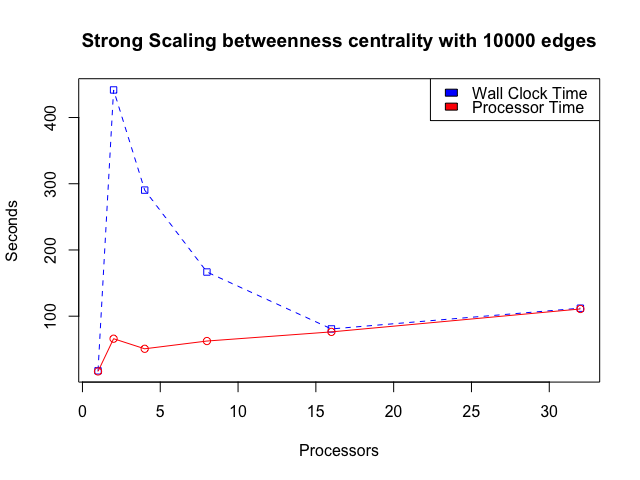
\includegraphics[width=0.9\textwidth]{figures/strong}
\caption{Strong scaling for betweenness centrality on a synthetic graph with
  10000 edges}
\end{figure}

\begin{figure}[h]
\centering
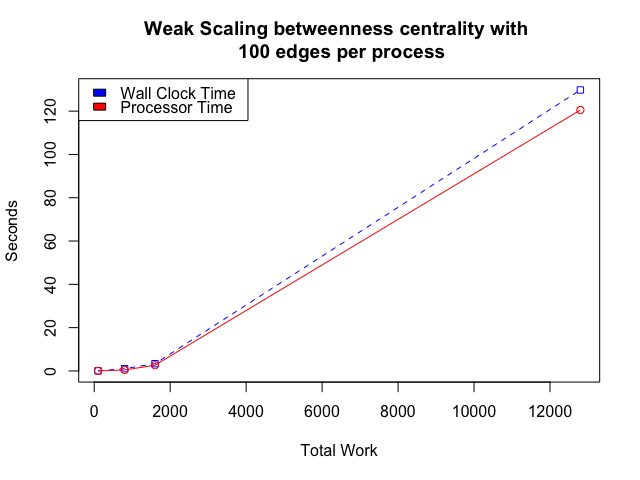
\includegraphics[width=0.9\textwidth]{figures/weak}
\caption{Weak scaling for betweenness centrality on a synthetic graph with
  100 edges per process}
\end{figure}



%% ============================= Results ============================= %%
\section{Results} % 4. experiments and results
\label{sec:results}
%     * Challenges of rendering large graphs
%     * Challenges of validating centrality
%     * Graphs of strong and weak scalability.
%     * Graphs of centrality found

Sam

\begin{figure}[h]
\centering
\includegraphics[width=0.9\textwidth]{figures/facebook}
\caption{Facebook betweenness centrality calculation}
\end{figure}

\begin{figure}[h]
\centering
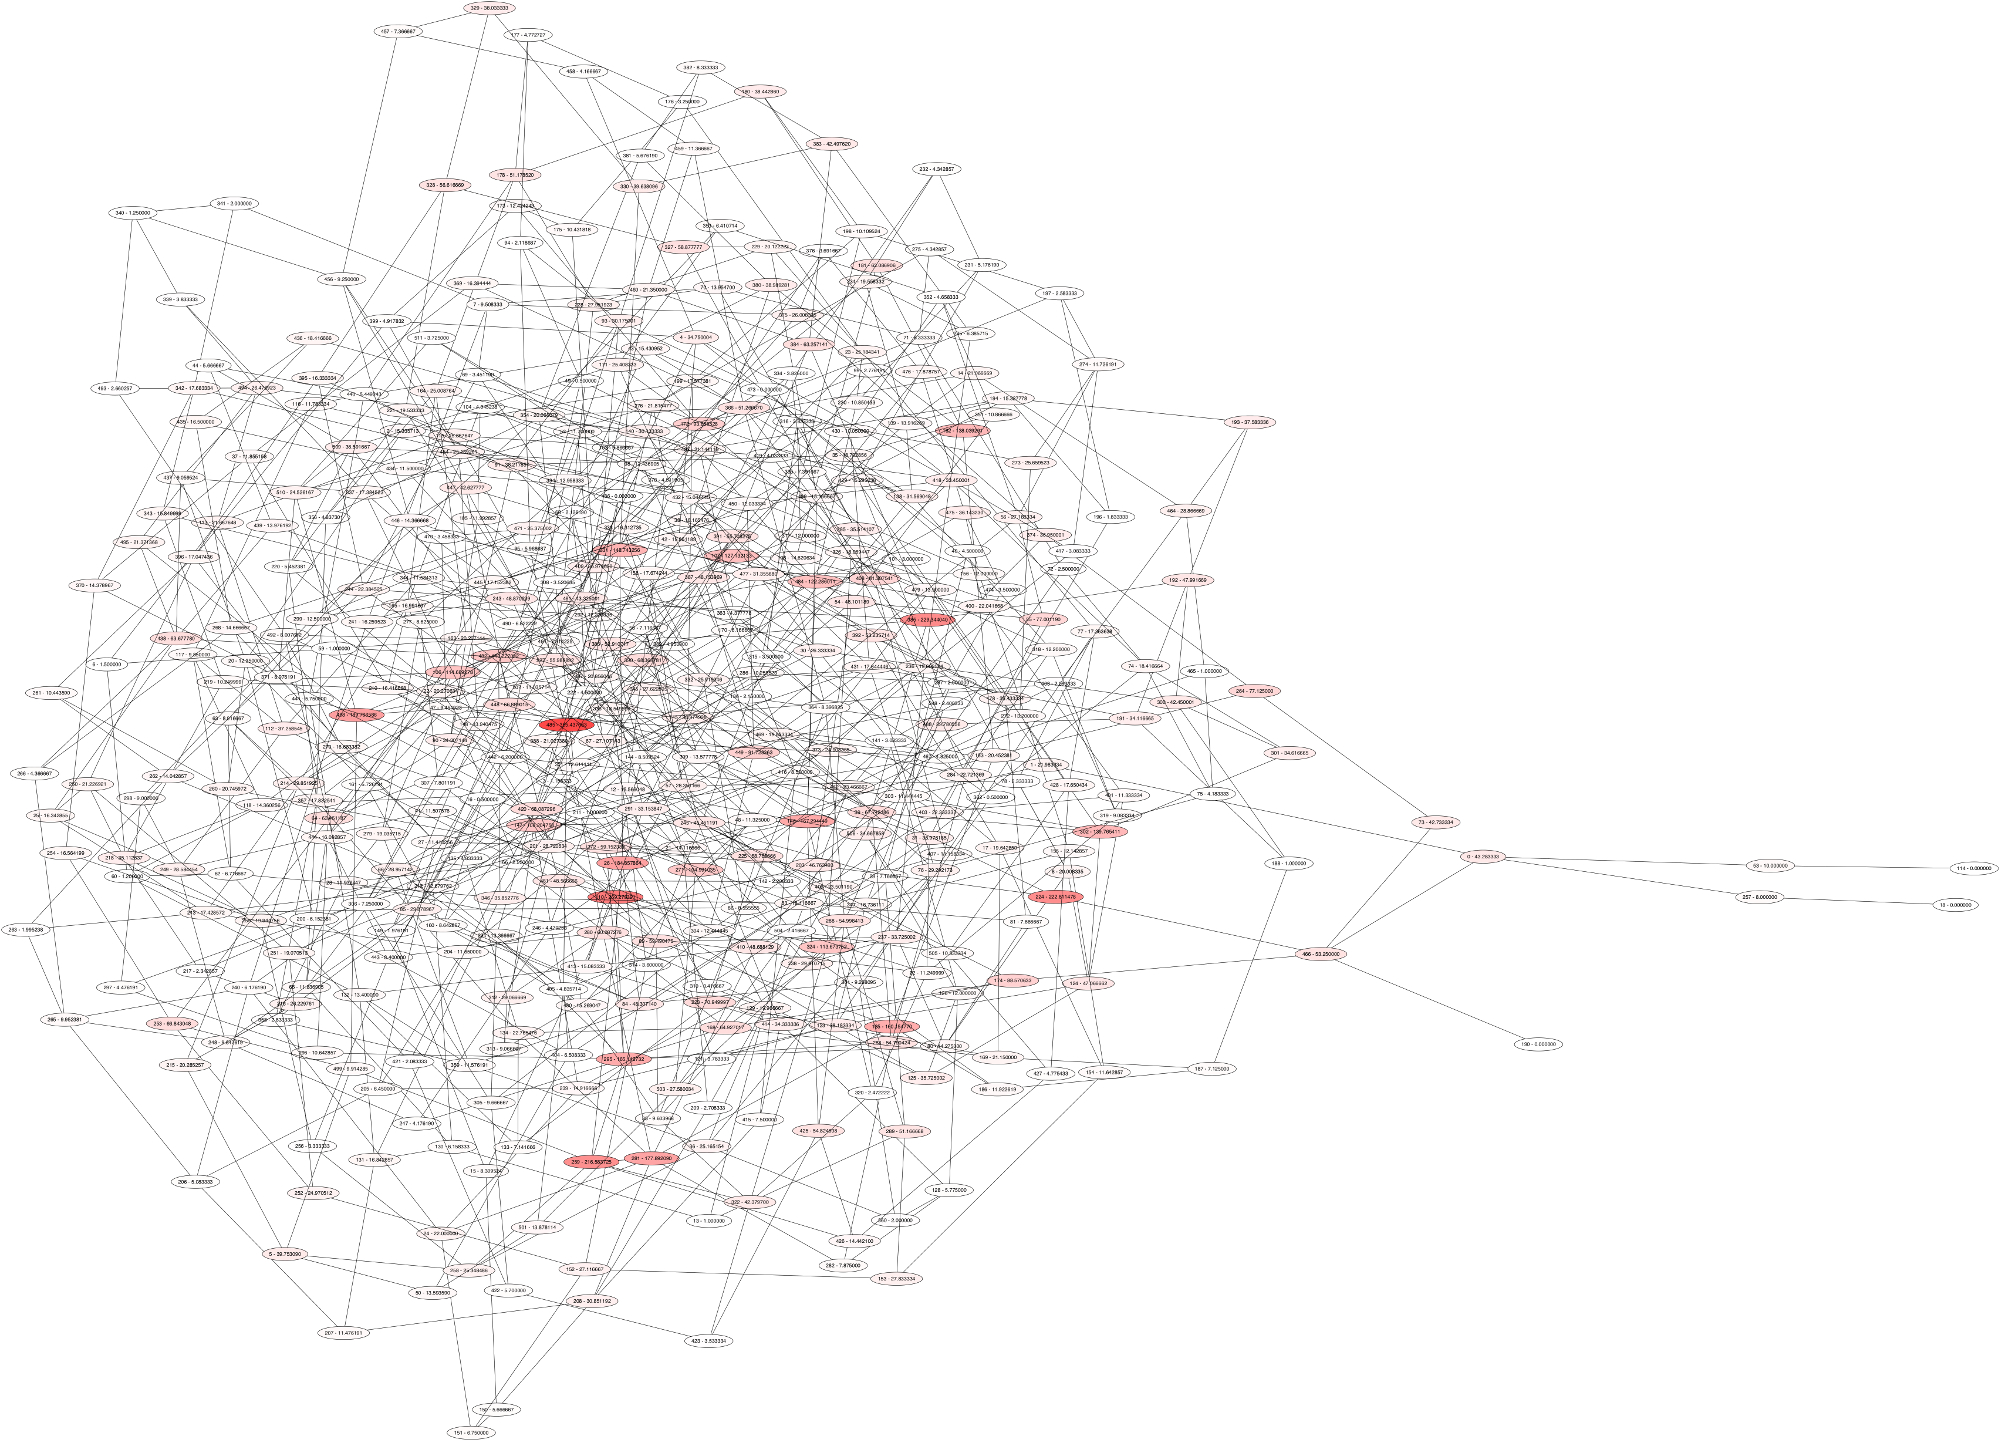
\includegraphics[width=0.9\textwidth]{figures/synthetic512_1}
\caption{Synthetic with 512 edges}
\end{figure}

\begin{figure}[h]
\centering
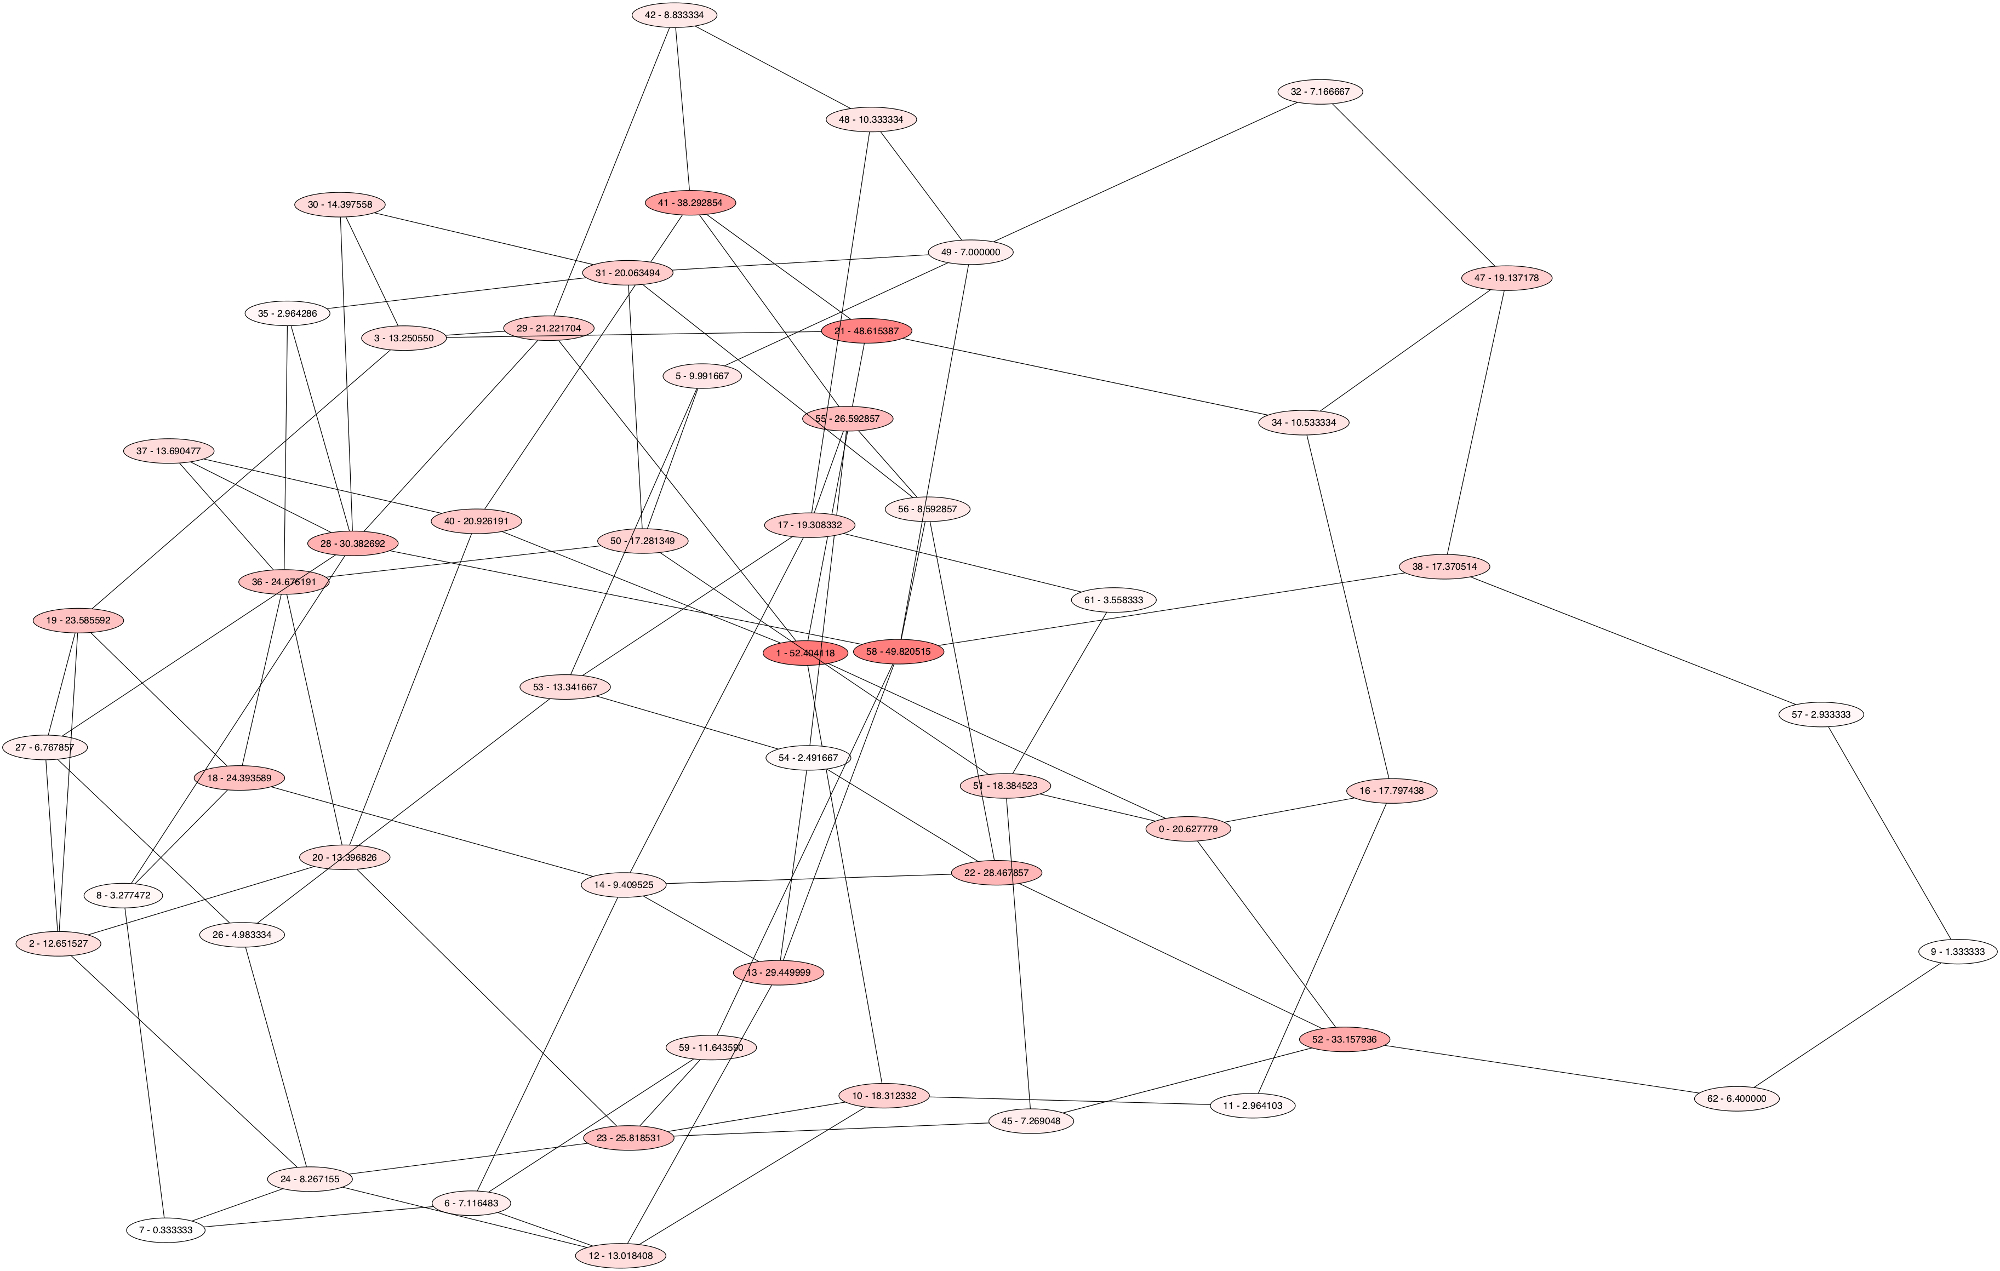
\includegraphics[width=0.9\textwidth]{figures/synthetic64_2}
\caption{Synthetic with 64 edges}
\end{figure}

%% ============================= Conclusion ============================= %%
\section{Conclusion} % 5. conclusions and future directions
\label{sec:conclusion}
%     * MPI and OpenMP really sped up the processing time



%% ============================= Future Work ============================= %%
\section{Future Work}
\label{sec:future-work}
%     * We could continue working to improve the running time and finding more
%       graphs to run it on
%     * We used a shared memory model, it would be interesting to try and break
%       up the graph into a distributed memory model.



%% ============================= Bibliography ============================= %%
\newpage
\bibliographystyle{acm}
\bibliography{references}



\end{document}
